Innerhalb des \ac{IoT} Core Brokers ist es möglich, Regeln zu definieren, die einzelne Nachrichten aus Topics in andere Dienste weiterzuleiten. Dazu müssen besagte Nachrichten selektiert werden, was mittels eines SQL Dialekts möglich ist. Eine beispielhafte Selektion könnte folgendermaßen aussehen: 


\begin{figure}[H]
\centering
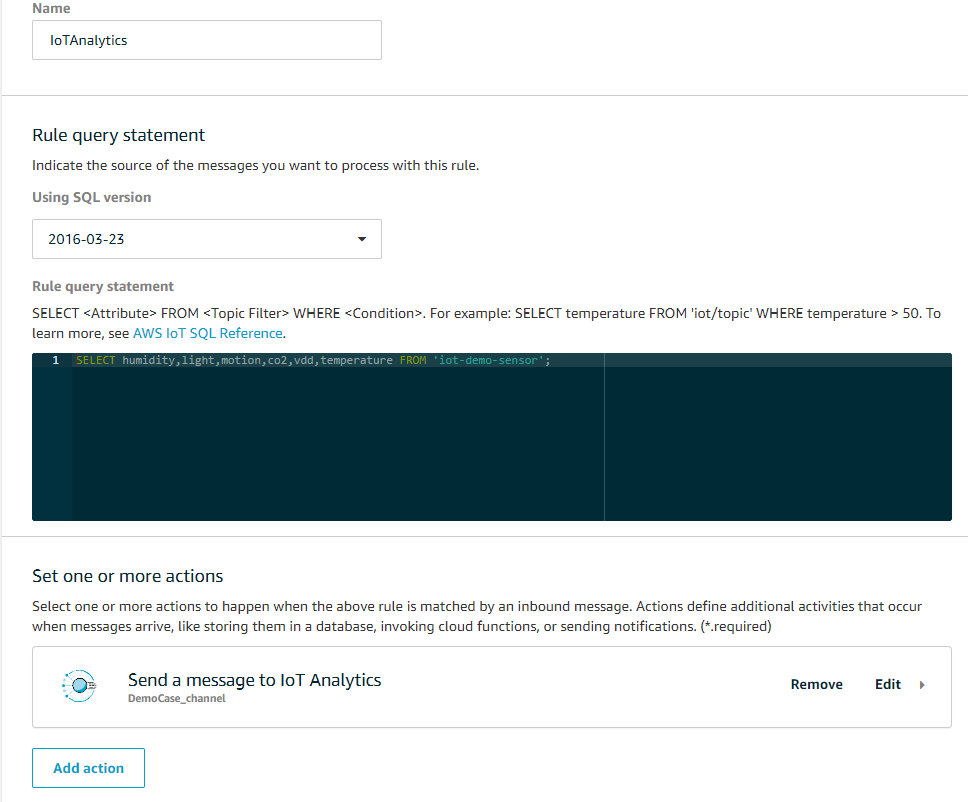
\includegraphics[width=\textwidth]{graphics/IoT-Rules-console.png}
\caption{Einstellung einer neuen Regel zur Weiterleitung an IoT Analytics}
\label{abb:IoTRulesExample}
\end{figure}

In \autoref{abb:IoTRulesExample} ist die Erstellung einer Weiterleitungsregel mit folgendem SQL Code zu sehen:
\lstset{language=SQL} 
\begin{lstlisting}
SELECT humidity,light,motion,co2,vdd,temperature 
FROM 'iot-demo-sensor'
\end{lstlisting}
Die Nachrichten aus dem Topic iot-demo-sensor werden dabei beispielhaft an IoT Analytics weitergeleitet.

\subsection{AWS IoT Analytics} \label{productselection:iotanalytics}
\AWSIOT Analytics ist ein Dienst der \AWSIOT Produktfamilie, der nach Aussage des Herstellers weitreichende Analysen von \ac{IoT} Daten, die beispielsweise via \AWSIOT Core geladen werden können, zulässt.
\begin{figure}[H]
\centering
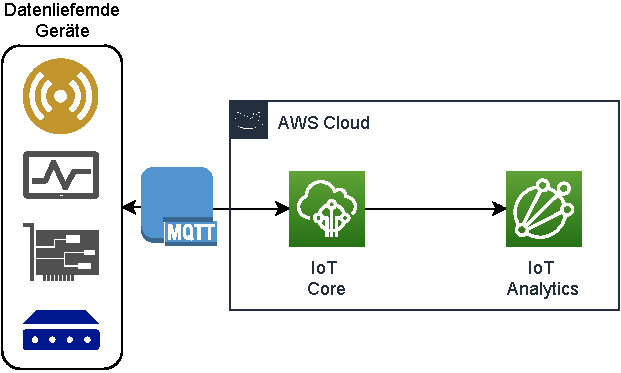
\includegraphics[width=\textwidth]{graphics/IoT-Analytics-general.pdf}
\caption{Grobarchitektur des Ablaufes für IoT Analytics}
\label{abb:GrobArchitekturIoTAnalytics}
\end{figure}
In \autoref{abb:GrobArchitekturIoTAnalytics} ist die Grobarchitektur und Verknüpfung mit anderen Diensten unter Annahme der Vorraussetzungen aus \autoref{chap:rahmendatenverarbeitung} gezeigt. Datenliefernde Geräte, wie beispielsweise Sensoren liefern Zeitreihen-Messwerte via dem \ac{MQTT} Protokoll an. Die Weiterleitung zu IoT Analytics erfolgt mittels einer eingerichteten Regel im \ac{IoT} Core Messagebroker, welche mittels eines Dialekts der SQL Sprache gewisse Topics vorselektiert oder alle Topics zulässt.

\Todo{IoT Events ansprechen (Schwellwerte)}

\subsection{Amazon Kinesis}
Amazon Kinesis ist im Gegensatz zu \AWSIOT Analytics nicht allein auf die Analyse von \ac{IoT} Daten spezialisiert. Kinesis eignet sich vielmehr für generelle Analysen von allerlei Streamingdaten. Zusätzlich ist Amazon Kinesis älter als \AWSIOT Analytics.

\begin{figure}[H]
\centering
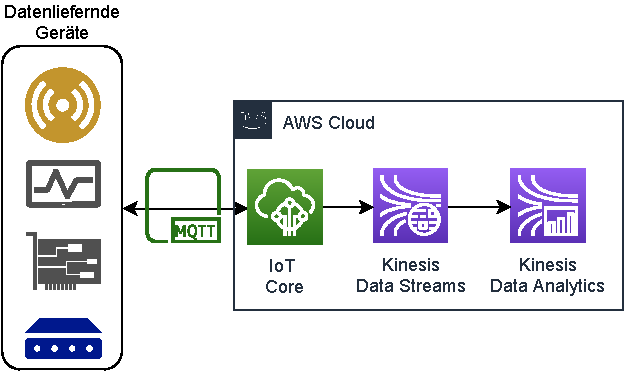
\includegraphics[width=\textwidth]{graphics/Kinesis-Analytics-general.pdf}
\caption{Grobarchitektur des Ablaufes für Kinesis Analytics}
\label{abb:GrobArchitekturKinesisAnalytics}
\end{figure}
In \autoref{abb:GrobArchitekturKinesisAnalytics} ist das Zusammenspiel der Dienste aus der Kinesis Familie mit anderen Diensten dargestellt. Angenommen werden dabei die in \autoref{chap:rahmendatenverarbeitung} erläuterten Rahmenbedingungen, weshalb \ac{IoT} Core als Message Broker eingesetzt ist. Wie in der in \autoref{productselection:iotanalytics} beschriebenen Architektur, muss auch hier für die Datenverarbeitung eine Regel im \ac{IoT} Core Broker angelegt werden, um relevante Nachrichten an Kinesis Data Streams weiterzuleiten.\footcite[Vgl.][]{AmazonWebServicesInc..o.J.}
\subsection{AWS Lambda}

\subsection{Produktauswahl}